%!TEX root = ../lections.tex
\subsection{Моды в линиях передачи}
Любая мода в лии передачи характеризуется поперечным волновым числом, а поперечное волновое число определяет продольное.

\begin{figure}[H]
	\centering
	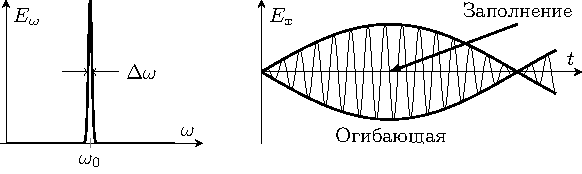
\includegraphics[scale=1.5]{img/lect3_ris8}
	\caption{Квазимонохроматический волновой пакет}
	\label{fig:lect3:8}
\end{figure}